\documentclass[border=6pt]{standalone}
\usepackage{tikz}
\usetikzlibrary{positioning}
\begin{document}
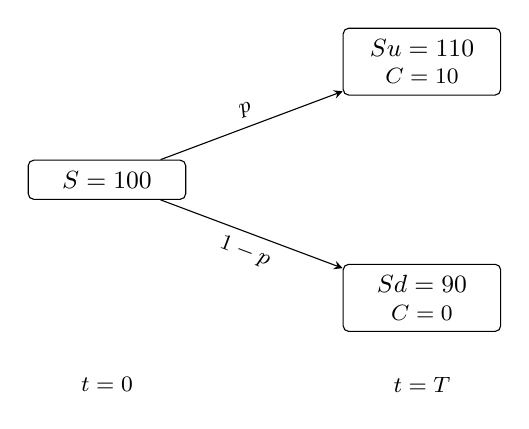
\begin{tikzpicture}[>=stealth,font=\small,
  node distance=10mm,
  nd/.style={draw,rounded corners=2pt,inner sep=4pt,minimum width=20mm,align=center}]
  \node[nd] (s0) at (0,0) {$S=100$};
  \node[nd] (su) at (4,1.5) {$Su=110$\\[-1pt]\footnotesize$C=10$};
  \node[nd] (sd) at (4,-1.5) {$Sd=90$\\[-1pt]\footnotesize$C=0$};
  \draw[->] (s0) -- node[above,sloped,font=\footnotesize] {$p$} (su);
  \draw[->] (s0) -- node[below,sloped,font=\footnotesize] {$1-p$} (sd);
  \node[font=\footnotesize] at (0,-2.6) {$t=0$};
  \node[font=\footnotesize] at (4,-2.6) {$t=T$};
\end{tikzpicture}
\end{document}
